% !TEX root = ../bachlor-arbeit.tex
\begin{tabular}{ll}
    \toprule
    Input: &
    Current spectrum $I'$, 
    Current design parameters $\mc D$\\
    Output: & 
    Improved design parameters $\mc D'$\\
    \bottomrule
\end{tabular}
\\
\\
The optimizer is at the core a Downhill-Simplex \cite{Nelder1965} tuning the continuous design parameters to minimize the mean-squared-difference between the current spectrum $I'$ and target spectrum $I$ we defined as 
$C_\s{mse}\qty(I, \, I')$.
However, the standard approach is unable to follow the physical constraints discussed in section \ref{sec:SASA} and has to be modified in that regard. To achieve this we can introduce a distance to the boundary $D$. Let $p$ be a single continuous parameter with lower bound $p^l$ and upper bound $p^u$, then

\begin{equation}
    D\qty(p, \, p^l, \, p^u) =
    \begin{cases}
        p^l - p, & \text{for } p < p^l\\
        0, & \text{for } p^l \leq p \leq p^u\\
        p - p^u, & \text{for } p^u < p
    \end{cases}
\end{equation}

\noindent
In this way one can penalize the simplex for stepping over the set boundaries by using a total loss $L$ which depends on the sum of all distances $D_i$

\begin{equation}
    L(I_\s{c}, \,I_\s{t}, \,p) =
    {\underbrace{%
    \vphantom{ \left(\frac{a^{0.3}}{b}\right) }
    C_\s{mse}(I_\s{c}, \, I_\s{t})}_{\text{find target}}}
    +
    {\underbrace{%
    \qty[\sum_i D\qty(p_i, \, p_i^l, \, p_i^u)]^3
    }_{\text{stay within bounds}}}\\
\end{equation}

The choice of exponent, 3 in this case, depends on how much the simplex should be penalized for stepping over a boundary. All our conditions are requirements for physical approximations and these approximations do no break completely when a boundary is only slightly violated. This justifies this approach where the simplex might step over a boundary but is then "pushed back" in the right direction. In figure \ref{fig:al:x_trans} we can see the optimizer in operation
\\

\indent
In the very left graph of figure \ref{fig:al:x_trans} at step 0 the 
optimizer has not jet tuned any parameters and the current and target spectrum are quite different. The blue target spectrum is in this case produced by a random stack from the validation data. This means there is a set of parameters which could reproduce this spectrum perfectly. By step 250 the optimizer has found a design which comes close to the original.

\begin{figure}[H]
    \centering
    \includegraphics[width=.9\linewidth]{al_x_trans}
    \caption{The fraction of transmitted light polarized in the $x$ direction over the wavelength in $\mu m$ at optimization steps 
    $(0, 50, 100, 250)$ left to right. Blue is the target spectrum $I$ and orange is the current spectrum $I'$.}
    \label{fig:al:x_trans}
\end{figure}

\begin{figure}[H]
    \centering
    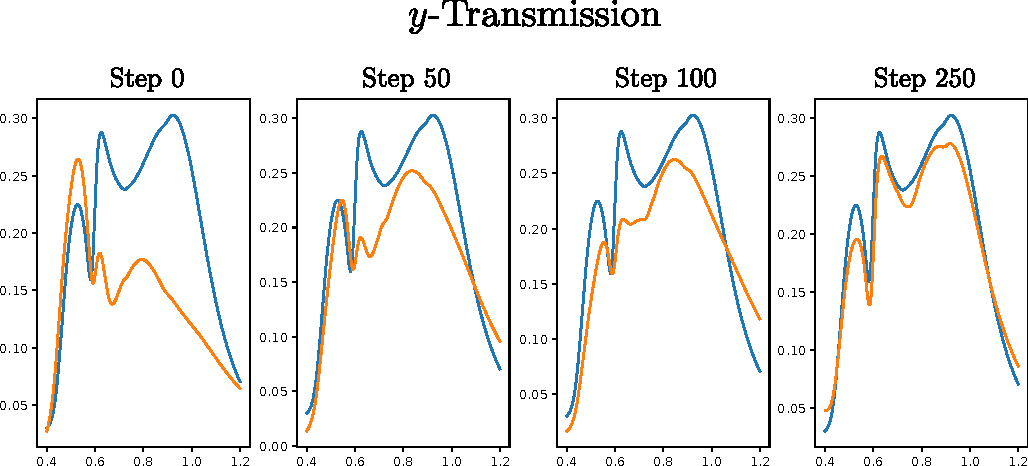
\includegraphics[width=.9\linewidth]{al_y_trans}
    \caption{The fraction of transmitted light polarized in the $y$ direction over the wavelength in $\mu m$. The optimization of the $y$ polarization is done simultaneous to the $x$ polarization shown in figure \ref{fig:al:x_trans}.}
    \label{fig:al:y_trans}
\end{figure}

To gain more insight we can consider how the parameters changed during the optimization as seen in figure \ref{fig:al:true_params}. As designed, the optimizer did not change the material and geometry parameters and they were chosen correctly by the Neural Network. This is in accordance with the high discrete accuracy seen in section \ref{sec:NN}. Some of the continuous parameters are close to the original but others like the rotation angle $\varphi$, second from the bottom, are completely different. This shows that even though we have removed the equivalent stacks described in figure \ref{fig:al:same_spec} there are still pairs of designs $\mc D_1, \mc D_2$ with different continuous parameters which produce very similar spectra $I \qty(\mc D_1) \simeq I \qty(\mc D_2)$ and these make it impossible for a network of this architecture to learn about the continuous parameters with good accuracy.

\begin{figure}[H]
    \centering
    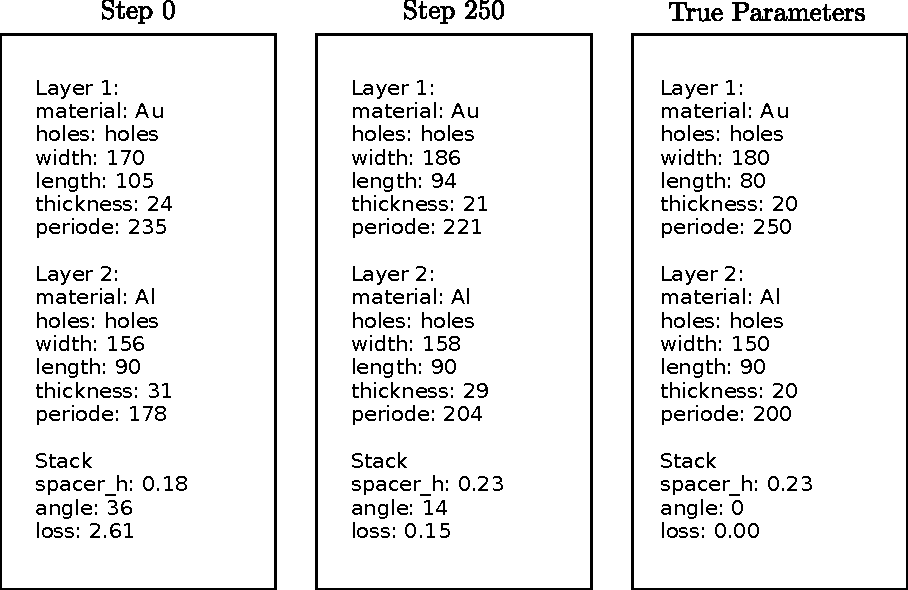
\includegraphics[width=.7\linewidth]{al_true_params}
    \caption{The design parameters $\mc D$ to the optimization shown in figure \ref{fig:al:x_trans} and \ref{fig:al:y_trans} at the beginning and end compared to the true parameters which produced the target spectrum.}
    \label{fig:al:true_params}
\end{figure} 